\section{System Description}

The 12-GeV Upgrade project scope is divided into three major systems:  
1) Accelerator System, 2) Physics System, and 3) Civil Construction System.  
The Physics System is further divided into four systems: 1) Hall A Upgrade, 
2) Hall B Upgrade, 3) Hall C Upgrade, and 4) Hall D. 

The Physics System equipment planned for the Upgrade project takes full 
advantage of the apparatus developed for the present program.  In Hall�B, 
the CEBAF Large Acceptance Spectrometer ({\tt CLAS}), which was designed to 
study multi-particle, exclusive reactions with its combination of large 
acceptance and moderate momentum resolution, will be upgraded to {\tt CLAS12} 
and optimized for studying exclusive and semi-inclusive reactions (emphasizing 
the investigation of so-called Generalized Parton Distributions and Transverse 
Momentum Dependent Parton Distributions) at high energy.  It will also be 
used for selected valence quark structure studies involving neutron ``tagging''
or polarized targets capable of supporting only very low beam current. Most 
importantly, the maximum luminosity will be upgraded from 
10$^{34}$~cm$^{-2}$s$^{-1}$ to more than 10$^{35}$~cm$^{-2}$s$^{-1}$.  The 
present time-of-flight counters, {\v C}erenkov detectors, and electromagnetic 
calorimeters will be retained, but the tracking system and other details of 
the central region of the detector will be changed to match the new physics 
goals. 

\section{Upgrade Hall B System Requirements}

The Hall B System shall meet the following requirements:

\begin{itemize}
\item 11 GeV polarized electrons beam,

\item Capability to run at luminosities of 10$^{35}$~cm$^{-2}$s$^{-1}$,

\item Operation of a longitudinally polarized target,

\item Capability to detect forward-going, high momentum particles from 
5 - 35$^\circ$,

\item Capability to detect recoil baryons at angles $>$35$^\circ$,

\item Large momentum range for the separation of electrons, pions, kaons, 
and protons.
\end{itemize}

The safety of personnel and equipment must be implemented in all phases of 
the {\tt CLAS12} detector upgrade, including R\&D, design, construction, and 
commissioning.

\section{Technical Approach to Meet the Upgrade Hall B System Requirements}

\subsection{Introduction}

The Hall B Upgrade System, also termed the {\tt CLAS12} detector, has evolved 
from the CEBAF Large-Acceptance Spectrometer, or {\tt CLAS}, to meet the 
basic requirements for the study of the structure of nucleons and nuclei with 
the CEBAF 12-GeV Upgrade.  A major focus of {\tt CLAS12} will be to determine 
the Generalized Parton Distributions (GPDs).  {\tt CLAS12} will be able to 
carry out the core program for the study of the internal dynamics and 3D 
imaging of the nucleon, and quark hadronization processes.  Both of these 
programs impose broad requirements for measuring multiple uncorrelated 
particles over a wide kinematic range with good resolution in momentum and 
angles.  These studies are carried out by measuring exclusive and 
semi-inclusive processes from hydrogen and nuclear polarized and unpolarized 
targets.  The access to GPDs at high photon virtuality requires use of large 
acceptance detectors capable of operating at high luminosity.  Moreover, a 
program to access GPDs requires use of polarized solid state targets that 
can only operate at a limited luminosity.  {\tt CLAS12} will provide the large 
acceptance to measure these processes well. 

{\tt CLAS12} makes use of many existing detector components.  Major new 
components include the superconducting torus coils that cover only the forward 
angle range, a new gas {\v C}erenkov counter for electron/pion separation, 
additions to the electromagnetic calorimeters, and the central detector.  In 
the following the modifications and new components are briefly described. 

{\bf Forward detector:}  The forward detector system will use several of the 
existing components: the low threshold gas {\v C}erenkov counters, all 
electromagnetic calorimeters, and the time-of-flight scintillators.  New 
components include the high threshold {\v C}erenkov counter, the torus magnet, 
and the forward drift chambers, which will cover an angle range from 5 to 
40$^\circ$.  The large drift chambers in {\tt CLAS} will be replaced by 
new detectors that will cover the 5 to 40$^\circ$ angle range.  Two of the 
existing detector systems, the time-of-flight system and the electromagnetic 
calorimeter system, need some upgrading to allow measurement of high 
momentum forward-going particles.  A pre-shower detector will be inserted in 
front of the existing {\tt CLAS} electromagnetic calorimeters to allow high 
energy photon detection and separation of single photons from neutral pion 
events.  Improved particle identification will be accomplished by several 
means: the timing resolution of the scintillation counters will be improved 
by adding an additional layer of scintillators with 40\% the widths of the 
existing layer and by using PMTs with better timing characteristics. 

{\bf Central detector (CD):}  A main component is a compact superconducting 
solenoid magnet, which has a triple function: it provides magnetic shielding 
of all tracking detectors from charged electromagnetic background, mostly 
M{\o}ller electrons and particles from secondary interactions. It provides 
the magnetic field for the momentum analysis of charged particles at large 
angles, and it provides the uniform 5-T field needed for the operation of a 
dynamically polarized solid state target.  The CD will detect charged 
particles from 35 to 125$^\circ$.  Several layers of silicon strip sensors 
will provide momentum analysis.  Particle identification is achieved by the 
combination of momentum analysis and time-of-flight measurements in the 
scintillation counters. 

{\bf Beamline and targets:}  Most of the existing beamline components will be 
re-used without changes.  This includes the photon tagger and pair 
spectrometer, the polarized photon instrumentation, a polarized target for 
photon experiments, and beam position and current monitors.

\subsection{Design Solutions to Fulfill the Requirements}

Requirement 1 (11-GeV beam capability) is satisfied by upgrading the 11-GeV 
Hall B beamline transporting electrons from the extraction region into the 
hall.  This scope resides within the Accelerating Systems Beam Transport 
WBS 1.3.4 and the Hall~B Upgrade Beamline WBS 1.4.2.5.

Requirement 2 (luminosity capability) requires a factor of 10 increase over 
the existing {\tt CLAS} luminosity.  This requirement drives two parts of the 
Hall B upgrade: the development of improved M{\o}ller electron shielding and 
changes in the drift chamber geometries.

\subsubsection{Improved M{\o}ller Electron Shielding}

The present luminosity limit for electron scattering experiments comes from 
M{\o}ller electrons produced in the target that interact either directly 
(first region of drift chambers) or through primary photons and the production 
of secondary particles in the support structures and torus coils with all 
three regions of drift chambers.  A large fraction of the M{\o}ller electrons 
affecting the first region are already shielded using a small toroidal magnet 
that does not block higher-energy charged particles from reaching the drift 
chambers, but which deflects the M{\o}ller electrons into the outer surface of 
massive shielding where they are absorbed.  This method allows {\tt CLAS} to 
operate at a luminosity of 10$^{34}$~cm$^{-2}$s$^{-1}$.  In the course of 
{\tt CLAS} operation of polarized targets using Helmholtz coils, it was 
determined that solenoidal shielding would be more effective at suppressing 
M{\o}ller electrons, because these electrons are `trapped' starting at their 
point of origin and they can be transported and dumped on the interior of a 
conical pipe, rather than on an exterior surface.  Subsequent simulations 
have validated this conclusion, and in addition showed that a strong 
solenoidal field with a large $\int Bdl$ gains another factor of $\sim$1.5 in 
luminosity increase, showing the luminosity increase is expected to be a 
factor of $\sim$3 in this approach.  However, use of solenoidal shielding is 
not practical in the current {\tt CLAS} except for experiments where the 
particles of interest are confined to small angles, since a solenoid magnet 
will block larger-angle particles that are needed for many experiments.  The 
technical solution for {\tt CLAS12} is to use solenoidal shielding where 
detector elements within the magnet bore cover the angles that would otherwise 
be blocked.  The discussion of Requirement 5 will elaborate further on this 
solution.  Requirement 4 (forward-angle range from 5 to 35$^\circ$), which 
specifies a minimum angle of 5$^\circ$ at 50\% acceptance in azimuthal angle 
for measured particles, means that the cone of M{\o}ller electrons must be 
confined to a significantly smaller angle so as to not flood the active 
detector volumes with low-energy tracks.  This requires that the $\int Bdl$ 
provided by the solenoid magnet downstream of the target must be sufficiently 
high to confine the M{\o}ller electrons into a small forward cone where they 
can be safely absorbed.  In detailed simulations of the field needed for this 
it was determined that a 5-T field was required with $\int Bdl$ =2.5~Tm 
downstream of the target, thus fixing the maximum solenoid field specification 
and its length.  The other limit of Requirement 4, a maximum angle of 
35$^\circ$, constrains the geometry of the massive components of the magnet.  
This requirement means that the downstream end of the solenoid needs to be a 
conical aperture allowing 35$^\circ$ particles from the cryo-target to pass 
through, thus fixing the downstream geometrical specification of the solenoid 
magnet.

\subsubsection{Drift Chamber Geometry}

Since improving the M{\o}ller shielding yields a factor of $\sim$3 increase 
in the luminosity limit, a remaining factor of 3-4 needs to be obtained 
relative to the existing drift chambers by reducing the solid angle of the 
drift chamber cell sizes in order to achieve Requirement 2.  The rate due to 
charged particles is approximately proportional to the drift chamber cell 
radius for a fixed distance between the target and the chamber.  The new 
Region~1 forward chamber will be at a 2.5 times larger distance from the 
target than the existing chamber (200~cm vs. 80~cm), which by itself will 
provide a luminosity limit increase of approximately a factor of 2.5.  
Further rate reduction (factor $\sim$2) is obtained by using a reduced time 
window due to the use of a higher field gradient, a slightly reduced wire 
spacing, and an additional reduction due to the better shielding of the large 
$\int Bdl$ of the solenoid field.  The 5-35$^\circ$ angle coverage in 
Requirement 4, together with the design choice of six-layer superlayers (to 
maintain the existing level of redundancy) and the wire spacing reduction, 
determines the forward drift chamber channel counts.  All three regions have 
112 channels/layer/sector, and there are 12 layers per region, which for six 
sectors yields a total channel count of 112$\times$12$\times$3$\times$6 = 
24,192 drift chamber cells.  Region~2 and Region~3 also need significantly 
lower rates, which are achieved by a combination of reduced production of 
secondary background particles and the reduced solid angle coverage due to 
the larger distance from the target, although this effect is smaller for the 
Region~2 (factor $\sim$1.7) and the Region~3 (factor $\sim$1.3) than for 
Region~1 (factor 2.5).  The combined increase in luminosity due to improved 
M{\o}ller electron shielding and the reduced sensitivity of the drift chamber 
cells was obtained in a detailed simulation and event reconstruction analysis 
with realistic physics background that resulted in comparable occupancies and 
reconstruction efficiencies for the {\tt CLAS12} and {\tt CLAS} configurations 
at 10 times higher luminosity for {\tt CLAS12}.

Requirement 3 (longitudinally polarized target) is satisfied by adapting the 
design of the existing polarized target to the geometry and conditions 
resulting from addressing Requirement 2 as discussed above.  Specifically, the 
polarized target cell operates in magnetic fields of high intensity, typically 
3 to 5~T, and high uniformity, and that is oriented along the beam axis.  The 
5-T solenoid field required to satisfy Requirement 2 can be used for this 
purpose, as long as the field uniformity required can be achieved.  The field 
uniformity required is 10$^{-4}$ within a cylindrical volume 3~cm in diameter 
and 10~cm in length.  This requirement sets the field uniformity specification 
for the solenoid magnet.

It should be noted that there are a number of differences between the existing 
polarized target and the {\tt CLAS12} polarized target.  The most important 
one is that the {\tt CLAS12} polarized target is fully contained in a 
cylindrical cryostat of 10-cm diameter and uses the 5-T field of the solenoid 
as the polarizing field.  It can thus be used in conjunction with the tracking 
detectors in the {\tt CLAS12} central detector.  The existing polarized target 
has its own large 5-T magnet coils integrated into the same vacuum system, and 
cannot be used together with the {\tt CLAS12} central tracking detectors and 
the solenoid magnet.  Also, the target mounting mechanism must be of a 
different geometry than the existing design.  All of these considerations are 
being taken into account.

Requirement 4 (capability to detect high-momentum particles from 5 to 
35$^\circ$) has been partially discussed under Requirement 2 above.  
High-momentum charged particles are detected by the combination of the 
forward part of the silicon vertex tracker, the drift chambers, the magnetic 
field from the torus magnet, and the time-of-flight scintillators.  The 
silicon vertex tracker is addressed in the discussion of Requirements 5 and 6.
The design solution for the drift chambers that satisfies Requirement 2 as 
discussed above is adequate to satisfy Requirement 4 as well.  The resolutions 
achievable with the wire spacing given and the planned drift chamber gas are 
consistent with the missing mass resolution needed to reconstruct missing 
particles.  The timing information from the time-of-flight counters is needed 
to perform the time-based tracking needed for the drift chamber analysis.  The 
magnetic field needed to momentum-analyze the detected charged particles is 
determined by the energy ranges of the particles and the geometries of the 
detectors and magnets.  The maximum field value and the profile of its 
intensity have been determined and specified by these considerations.  The 
azimuthal angle coverage extends down to polar angles of 5$^\circ$ where it 
is 50\% of 2$\pi$.  The minimum angle coverage in the {\tt CLAS} standard 
configuration is limited to about 10$^\circ$ and covers a smaller range in 
azimuthal angle.  The fall-off in integrated field strength is also 
significantly different from the existing torus, and is well-matched to the 
momentum spectra of the charged particles anticipated.

Neutral particles at high energies will be detected using the forward 
calorimeters.  Because of the increased beam energies, neutral pions at high 
momentum are no longer able to be detected with the existing {\tt CLAS} 
forward calorimeter, necessitating the addition of the pre-shower calorimeter 
that has a finer-grained readout that can resolve the two photons from  
neutral pion decay.  The parameters of the pre-shower calorimeter have been 
optimized for this purpose, determining the specifications for the device.  
Neutrons will be detected in the pre-shower calorimeter, as well as the 
existing calorimeter, increasing the overall efficiency of neutron detection.  
The increase in granularity also translates into an improved angular 
resolution for neutrons detected in the pre-shower calorimeter.  While the 
design was optimized for neutral pions, as driven by Requirement 4, the 
improvement in neutron detection is an important additional benefit.

It should be noted that the fulfillment of Requirement 4 is supported in an 
important way by Requirement 6 (particle identification over a wide momentum 
range), since `detecting' a particle generally requires a determination of 
the particle type.

Requirement 5 (detecting recoil baryons at large angles) is addressed by the 
central detector package.  This detector set is mounted inside the solenoid 
magnet.  It includes the barrel portion of the silicon vertex tracker, a 
time-of-flight array, and the provision of space for a compact detector for 
neutral particle detection.  Determination of the charged particle momentum 
is performed by recording the hit positions of the helical trajectories in the 
silicon vertex tracker in the solenoid magnetic field.  Identification of the 
particle type is performed by combining the momentum information with the time 
as measured by the time-of-flight system.  The parameters of the barrel 
portion of the SVT, such as strip pitch, level of redundancy, and thickness of 
materials are chosen to optimize detection of recoil particles. 

Requirement 6 (particle identification over a large range in momentum) has 
been addressed by a number of design choices.  A second gas {\v C}erenkov 
counter that has a higher pion detection threshold was added to increase the 
range of electron-pion separation to approximately 5~GeV.  This high threshold 
{\v C}erenkov counter (HTCC), which is located in front of the Region~1 drift 
chamber, is designed to have minimal mass to reduce its impact on the tracking 
information.  To further reduce the impact of this added mass, the forward 
part of the Silicon Vertex Tracker (SVT) was added, which samples tracking 
information before the particles arrive at the HTCC and provides a track 
vector to match to the forward drift chambers. 

The location of the HTCC just downstream of the target and before the torus 
magnet and the drift chamber system is a natural choice that does not add 
much length along the beam line to the overall length of {\tt CLAS12}.  The 
relative positioning of the solenoid and the torus magnet is largely 
determined by the out-of-plane forces the transverse magnetic field of the 
solenoid exerts on the current in the torus coils.  The transverse magnetic 
field must be limited to $<$50~G to limit distortions of the torus coil 
panels to acceptable levels, which requires a distance of at least 220~cm 
from the solenoid center (target center) to the torus coils.  This space is 
ideally suited for inserting the HTCC detector, which requires an overall 
length of approximately 150~cm beginning 30~cm downstream of the target center.
           
A second component of the particle identification scheme is to use the 
existing panels of time-of-flight scintillators in the forward region and 
to add a second layer with smaller scintillator widths and new photomultiplier 
tubes to construct new time-of-flight detectors with better timing resolution.
This requirement is the basis for the specifications for their performance.  A 
third component is the time-of-flight counters within the solenoid magnet, 
part of the central detector, which was mentioned in the discussion of 
Requirement 5.  Identification of the particles in this lower-momentum region 
is important and it drives the performance requirements for these detectors.

Finally, as already discussed for Requirement 4, the pre-shower calorimeter is 
required to identify neutral pions at the highest energies.  While it has been 
optimized for this purpose, it will also improve the identification of 
electrons, pions, and neutrons. 

\section{Superconducting Torus and Solenoid Magnets}

The {\tt CLAS12} spectrometer system (see Fig.~\ref{magnet1}) contains two 
superconducting magnets, a 5-T solenoid magnet and a toroid magnet with a 
maximum  field of 2.5~T.  The two magnets provide magnetic analysis of charged 
particles in the large-angle range and the forward-angle range, respectively. 
The magnets are separated in space by a distance of about 1.5~m and their 
respective fields are partially overlapping.  Owing to its symmetry properties,
the toroid field drops rapidly with distance and has virtually no impact on 
the solenoid magnet.  In particular, since its field is zero on the beam axis, 
it does not affect the homogeneity of the solenoid magnet in the critical 
target region.  The solenoid  field drops more slowly with distance and exerts 
a measurable force on the coils of the toroid magnet that must be taken into 
account in the mechanical design of the toroid magnet.  At the closest 
distance between the solenoid and toroid magnets, the coil deflection is about 
1.3~mm. Since the solenoid field is cylindrically symmetric, it affects all 
six toroid coils in the same way.

%%%%%%%%%%%%%%%%%%%%%%%%%%%%%%%%%%%%%%%%%%%%%%%%%%%%%%%%%%%%%%%%%%%%%%%%%%%%%%
\begin{figure}[htbp]
\vspace{11.5cm}
\special{psfile=CD3_CLAS12.eps hscale=30 vscale=30 hoffset=0 voffset=45}
\special{psfile=magsys1.ps hscale=38 vscale=31 hoffset=250 voffset=155}
\special{psfile=magsys2.ps hscale=38 vscale=31 hoffset=250 voffset=45}
\special{psfile=magsys3.ps hscale=38 vscale=31 hoffset=250 voffset=-65}
\caption{\small{(Left) {\tt CLAS12} showing the solenoid (brown) on the  
left and the torus (gray) between the drift chambers.  (Right) {\tt CLAS12}
transverse magnetic field as a function of $z$ for polar angles of 10$^\circ$,
20$^\circ$, and 30$^\circ$ at $\phi$=0$^\circ$.  The torus transverse field
becomes weaker with increasing angle, while the solenoid transverse field
increases in strength.}}
\label{magnet1}
\end{figure}
%%%%%%%%%%%%%%%%%%%%%%%%%%%%%%%%%%%%%%%%%%%%%%%%%%%%%%%%%%%%%%%%%%%%%%%%%%%%%%

\vfil
\eject

\subsection{The {\tt CLAS12} Toroid}

{\tt CLAS12} is a magnetic spectrometer based on six super-conducting coils 
arranged around the beam line to produce a field primarily in the $\phi$ 
direction (see Fig.~\ref{magnet2}).  The choice of this configuration leads 
to an approximate toroidal field distribution around the beam axis.  It has
been driven by the necessity of satisfying the precise requirements determined 
by the physics program of:

\begin{itemize}

\item uniform coverage of a large angular and momentum range for charged and 
neutral particles;

\item good momentum and angular resolution; due to the Lorentz boost, the 
average momentum increases with decreasing emission angle from the target and 
the relative momentum resolution ($\Delta p/p$) has to improve in the forward 
direction to maintain a constant absolute resolution;

\item good particle identification; the open structure of the toroid allows 
for long path lengths for charged and neutral particles for good particle 
identification through time-of-flight measurements, high luminosity, and 
counting rate capability: expected operating luminosity is 
$1 \times 10^{35}$~cm$^{-2}$s$^{-1}$.

\item low background from electromagnetic processes (M{\o}ller electrons; 
$e^+e^-$ pairs, etc.);

\item symmetry around the beam axis;

\item compatibility with the operation of a polarized target; the field 
symmetry of a toroid provides full field compensation on the magnetic 
symmetry axis and allows operation of polarized targets near the beam axis 
with their own magnetic holding fields.

\end{itemize}

%%%%%%%%%%%%%%%%%%%%%%%%%%%%%%%%%%%%%%%%%%%%%%%%%%%%%%%%%%%%%%%%%%%%%%%%%%%%%%
\begin{figure}[htbp]
\vspace{7.5cm}
\special{psfile=magnet_view2.eps hscale=27 vscale=27 hoffset=25 voffset=0}
\special{psfile=magnet_view1.eps hscale=27 vscale=27 hoffset=240 voffset=0}
\caption{\small{The {\tt CLAS12} toroid magnet.  The left panel shows the
toroid model by itself and the right panel shows the toroid with the
full set of drift chambers attached.}}
\label{magnet2}
\end{figure}
%%%%%%%%%%%%%%%%%%%%%%%%%%%%%%%%%%%%%%%%%%%%%%%%%%%%%%%%%%%%%%%%%%%%%%%%%%%%%%

The toroid configuration offers a field-free region around the target and a 
magnetic field that is always transverse to the particle trajectory.  The first
characteristic allows the installation of a polarized target with no 
interference between the target and detector magnetic fields.  In addition, 
since the $\phi$ pattern of the event is preserved in the toroidal magnetic 
field, the determination of the azimuthal angle $\phi$ is decoupled from the 
measurement of the polar angle $\theta$ and momentum $p$.

The six coils have been shaped to give the desired $\int B dl$, and therefore, 
the requested resolution as a function of $\theta$.  The coil-operating 
temperature of 4.5~K is maintained by a forced flow of super-critical
liquid helium supplied by the Central Helium Liquefier (CHL).  The total
stored electromagnetic energy at the nominal operating current is 16~MJ.
Table~\ref{mag_parms1} shows the main parameters of the toroid coils.

%%%%%%%%%%%%%%%%%%%%%%%%%%%%%%%%%%%%%%%%%%%%%%%%%%%%%%%%%%%%%%%%%%%%%%%%%%%%%%
\begin{table}[htbp]
\begin{center}
\begin{tabular} {||l|c||} \hline \hline
Conductor                         & NbTi \\ \hline
Configuration, overall dimensions & Six trapezoidal sections \\ \hline
Radial thickness                  & 294 mm \\ \hline
No. of double pancakes in section & 1 \\ \hline
No. of turns in double pancake    & 2$\times$140 = 280 \\ \hline
Conductor length (one section)    & 2.43 km \\ \hline
Conductor length (torus)          & 14.56 km \\ \hline
Torus inductance                  & 3.12 H \\ \hline
Conductor current                 & 3150 A \\ \hline
Amp-turns (one section)           & 0.882 mA \\ \hline
Amp-turns (torus)                 & 5.3 mA \\ \hline
Stored energy (torus)             & 15.5 MJ \\ \hline
Max. field (at the winding)       & 4.6 T \\ \hline
$\int B dl$ ($\theta$=40$^\circ$) & 0.517 Tm \\ \hline
$\int B dl$ ($\theta$=5$^\circ$)  & 3.32 Tm \\ \hline
$\int B dl$ ($\theta$=20$^\circ$) & 1.43 Tm \\ \hline \hline
\end{tabular}
\end{center}
\caption{\small{Parameters of the torus reference winding.}}
\label{mag_parms1}
\end{table}
%%%%%%%%%%%%%%%%%%%%%%%%%%%%%%%%%%%%%%%%%%%%%%%%%%%%%%%%%%%%%%%%%%%%%%%%%%%%%%

\subsection{The {\tt CLAS12} Solenoid}

Solenoid magnets provide an ideal field distribution for the analysis of 
particle trajectories in the central region, where the bending power of the 
solenoid field is at a maximum.  In {\tt CLAS12} the choice of a 5-T strong 
solenoid field has been driven by the necessity of satisfying precise 
requirements determined by the physics program of: 

\begin{itemize}

\item large opening for charged and neutral particles in the forward 
hemisphere; high momentum forward-going particles will not experience high 
enough transverse field components from the solenoid field and must be 
momentum-analyzed in the toroidal field located downstream of the solenoid 
magnet.  An opening in $\theta$ up to $\pm$40$^\circ$ is required;

\item good charged particle momentum resolution in a limited radial space for 
polar angles $\theta$ from 35$^\circ$ to 125$^\circ$ and momentum range from 
0.3 to 1.3~GeV;

\item operation of a dynamically polarized target; requires a high magnetic 
field with field non-uniformity over the target volume of 
$\Delta B/B < 10^{-4}$ ;

\item high luminosity operation; the solenoid field offers an effective 
shield of the sensitive tracking detectors against the very high background of 
M{\o}ller electrons.  The longitudinal field keeps low-energy electrons (and 
positrons) away from the sensitive tracking detectors and guides them into 
areas where they can dump their energy in specially designed heavy metal 
(lead or tungsten) absorbers;

\item compensation of the solenoid magnetic stray field; the {\tt CLAS12} 
detector setup requires locating magnetic sensitive photon detectors in areas 
surrounding the solenoid magnet.  The magnetic field drops only slowly with 
radial distance, and must be shielded with additional superconducting 
compensation coils built directly into the same cryostat as the solenoid coils 
and powered in series with the main coils.  The field in the sensitive regions 
can be compensated to values below 25~G.

\end{itemize}

The solenoid magnet provides a strong effective field needed for a 
dynamically polarized solid-state target.  At the same time, the solenoid 
field is used for particle tracking and momentum analysis by measuring the 
trajectory of charged particle in the field with a high-resolution tracking 
detector.   Fig.~\ref{magnet3} shows the magnetic field distribution
associated with the solenoid design.

%%%%%%%%%%%%%%%%%%%%%%%%%%%%%%%%%%%%%%%%%%%%%%%%%%%%%%%%%%%%%%%%%%%%%%
\begin{figure}[htbp]
\centering
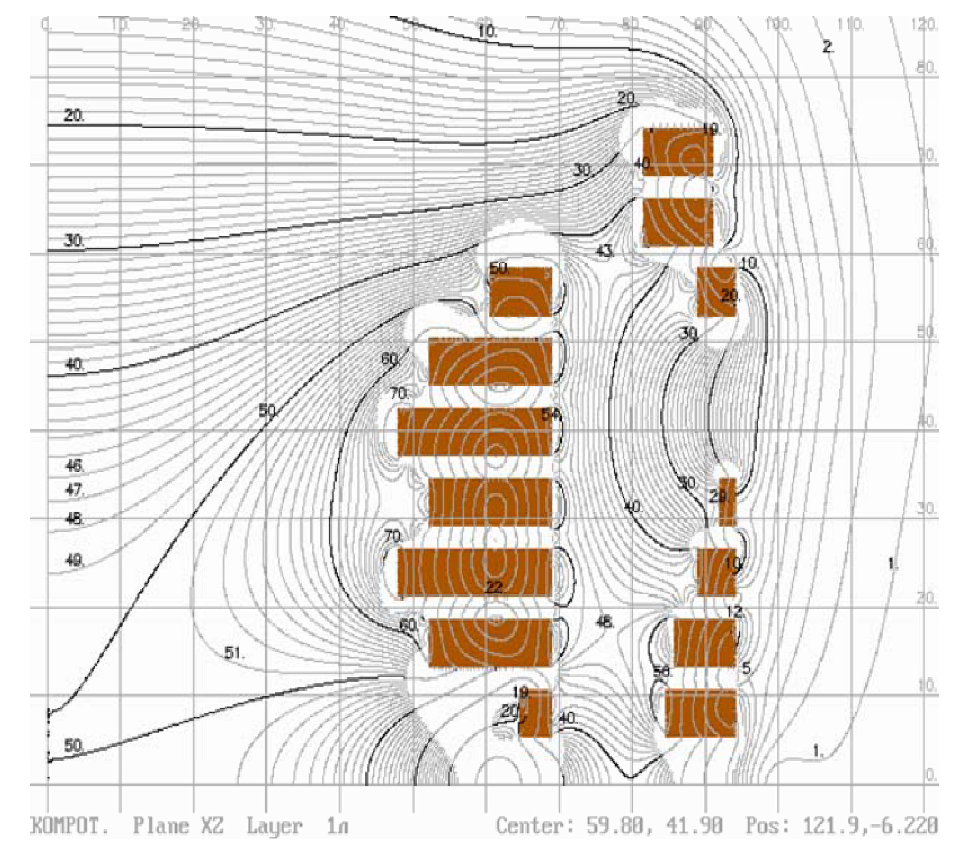
\includegraphics[width=0.5\textwidth]{sol_field1.ps}
\includegraphics[width=0.5\textwidth]{sol_field2.ps}
\caption{\small{(Top) One ``quadrant'' of the 5-T superconducting solenoid 
coil system.  Shown is the inner main coil and the outer compensation coil.  
Also shown are lines of constant field.  (Bottom) The large distance field 
distribution, showing the effect of the compensation coil.  At a 1.5~m radial 
distance at $z$=0 from the symmetry axis, the field strength is below 15~G. 
(Coordinates given in cm.)}}
\label{magnet3}
\end{figure}
%%%%%%%%%%%%%%%%%%%%%%%%%%%%%%%%%%%%%%%%%%%%%%%%%%%%%%%%%%%%%%%%%%%%%%

The total $\int B dl$ on the magnetic axis is 6.0~Tm and the stored energy at 
the 5~T central field is 25~MJ.  The main parameters are given in the 
Table~\ref{mag_parms2}.

%%%%%%%%%%%%%%%%%%%%%%%%%%%%%%%%%%%%%%%%%%%%%%%%%%%%%%%%%%%%%%%%%%%%%%%%%%%%%%
\begin{table}[htbp]
\begin{center}
\begin{tabular} {||l|c||} \hline \hline
\multicolumn{2} {||l||} {Main winding} \\ \hline
Inner diameter      & 943 mm \\ \hline
Aperture            & 780 mm \\ \hline
Max. outer diameter & 1300 mm \\ \hline
Length              & 1225.6 mm \\ \hline
Number of turns     & 4000 \\ \hline \hline
\multicolumn{2} {||l||} {Shielding winding} \\ \hline
Min. inner diameter & 1636 mm \\ \hline
Outer diameter      & 1804 mm \\ \hline
Length              & 1685.2 mm \\ \hline
Number of turns     & 1800 \\ \hline \hline
\multicolumn{2} {||l||} {General} \\ \hline
Inhomogeneity in working area & 5 ppm \\ \hline
Field in center               & 4.5 -- 5.0 T \\ \hline
Field at PMTs                 & $<$18 G \\ \hline
Max. field at the winding     & 6.8 -- 7.5 T \\ \hline
Nominal operating current     & 2399 -- 2665 A \\ \hline
Inductance                    & 6.95 H \\ \hline
Stored energy                 & 19.99 -- 24.68 MJ \\ \hline \hline
\end{tabular}
\end{center}
\caption{\small{Parameters of the solenoid reference winding.}}
\label{mag_parms2}
\end{table}
%%%%%%%%%%%%%%%%%%%%%%%%%%%%%%%%%%%%%%%%%%%%%%%%%%%%%%%%%%%%%%%%%%%%%%%%%%%%%%
